
\chapter{Introduction}
Consider the images shown in Figure 1, they are two images from the Government of Prince Edward Island website of historical aerial photography[6] both taken in 1935. We can gain tremendous amounts of information by comparing historical images against present day images or various images from different points in history. Even Google Map’s satellite imagery[2] gives everyone access to recent satellite photographs of most anywhere in the world. These can be compared against historical aerial photographs to monitor development, city growth, changes in crops, erosion of coast line and any number of changes and geographical evolutions through the ages. 
A major challenge however when comparing two images containing portions of the same thing is to align the photos. This alignment process can be tricky, considering again Figure 1, the two photos contain the same shoreline but to best compare the photos we need to rotate, deform and translate one photo so the same parts of each image fit over one another. In computer vision terms this process is known as image registration. 
If you consider that for Prince Edward Island this is especially tricky. Naive approaches like aligning the geometric shapes formed by the various farm fields with one another may work for some fields but for others they may change too much from one photo to the next (especially given a time period of more than 80 years). Aligning the shore line can be difficult for a number of reasons but in PEI the shoreline has changed in the last 80 years and also from photos given the shallow waters it can be tricky to decide where the shore actually is, especially at low or high tide from a photograph taken at altitude.
\begin{figure}
    \centering
    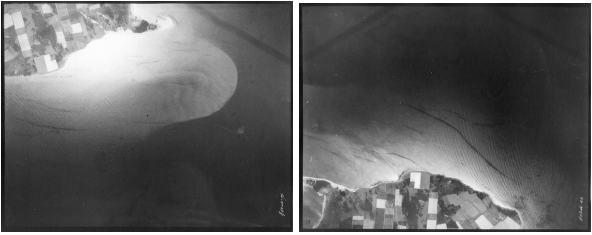
\includegraphics[width=3.0in]{figs/test}
    \caption{Example historical aerial images}
 
\end{figure}

Figure 1: Two aerial photographs overlapping the same portion of Prince Edward Island taken in 1935. The photos are not aligned (nor in the same orientation), however looking closely you can match the same parts in one image with the other. 
 
 


\section{Problem}

Estimating correspondences between images is one of the the fundamental problems in computer vision with applications ranging from large-scale 3D reconstruction to image manipulation and semantic segmentation. It is also difficult for a person to estimate the changes between the aerial images.\\       
 When we try to align the two aerial images with our eyes, first we might find an interesting point in one image that we can find in the other image. 'The island' will be the interesting feature in Figure 1.1. compare the pair image, we will have to rotate one image and shift one image a little bit to get the same orientation, and if we do this for a few more interesting points we could discover one image is bigger than the other (or more zoomed in), so we shrink one image down a little bit and continue trying to align these interesting points we have identified. Eventually we can match two images as best as we can do. Some of the interesting points may have changed slightly - like a road was repaved in a slightly different way, or a farm field is close but maybe it appears a little larger in one image and maybe the shoreline has eroded a small amount. There may not be a perfect answer but eventually you get the best alignment.That is how we approach this problem as an person. In computer vision, there are few solutions to approach this the image alignment problem.  \\
  Traditionally, correspondences consistent with a geometric model such as epipolar geometry or planer affine transformation , are computed by detecting and matching local features (such as SIFT), followed by pruning incorrect matches using local geometric constraints and robust estimation of a global geometric transformation using algorithms such as RANSAC \cite{fischler1981random}. \\
In this work we uses the convolutional neural networks(CNN) architecture that builds on the traditional approach and mimics the search for interesting points (local features) by using powerful convolutional neural networks, further a neural network can be used to find an affine transformation matrix that aligns one image with the other. Instead of the traditional algorithms such as SIFT and RANSAC. The neural network approach has a advantages over existing algorithmic approaches.\\
Speed is one of the advantages of the neural network approach. A neural network does all the learning up front, this is timely but most only be done once. When the network is trained then computing the alignment of two images is very quick. We need just apply the operations outlined by the neural network once, no training or iterations required. Compare this with an approach such as SIFT, the algorithm uses for detecting the local features from given images and followed by RANSAC\cite{fischler1981random}, the algorithm to estimate parameters from given features points.\\
Reuse is other advantages of the neural network approach. Once the NN is trained we can use it over and over again. Further to find interesting points in an image we can make use of a NN model that has already been used for image processing purposes. Finding image features is a common task and so to achieve this part of our solution we need not retrain any neural networks. We can make use of an existing and highly powerful NN to do this for us.\\
The SIFT and RANSAC solution is expensive. It has to go through the whole algorithm every time when we provide a new pairs of images, with machine learning solution, the neural networks can learn the transformation over times with labelled data, it may take longer when it is on training, but it doesn't have to start with zero knowledge every time to find the solutions, the more and well the neural network is trained, the faster and more accuracy the solution will get.\\
 A disadvantage of the neural network approach is that we are doing supervised learning. As we will outline later in the thesis, supervised learning requires a large dataset containing labelled answers. For the labelled answer means. We develop the way to harvest the aerial images and generating sub image pairs with affine transformation without the noise, and develop the labelled answer means the affine transformation matrices between the aerial image and the target images. 

\section{Interesting(Machine Learning solution)}
The rest of this paper will outline the machine learning solution that will allow us to align images.
The machine learning solution involve a dataset with paired satellite images. Taking one image and applied it with an affine transformation to generating new paired images, and label the pair images with the affine transformation.\\ 
Other part of the solution is to construct convolutional neural network to run the algorithms instead of using SIFT or RANSAC to align the images. The solution model includes feature extraction, that find the key features in given images. Feature normalization, that normalize the features that has been extracted from the images. Feature correlation that find the correlation between features. Feature Regression which will return the affine transformation between paired images.\\
\begin{figure}
\centering
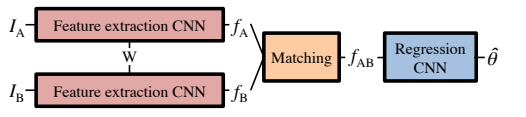
\includegraphics[width=3.0in]{figs/cnn_model}
\caption{The model that we use to produce an affine transformation matrix, $\theta$, from two source images, $I_A$ and $I_B$. \cite{Rocco17}}
\end{figure}
\begin{center}
affine  matrix = $\begin{bmatrix}
0&1&tx \\
1&0&ty
\end{bmatrix}$
\end{center}

\subsection{Feature extraction}
The feature extraction, which uses a standard CNN architecture. A CNN without fully connected layers takes an input image and produces a feature map $f \in R^{h*w*d}$, which can be interpreted as a $h * w $ dense spatial grid of d-dimensional local descriptors. For feature extraction we used the VGG-16 networks \cite{simonyan2014very}, cropped at the $ pool4 $ layer (before ReLU unit), followed by per-feature L2-normalization.The feature extraction network is duplicated and arrange in a Siamese configuration such that two input images are passed through two identical networks with share parameters.
\begin{figure}
	\begin{center}
	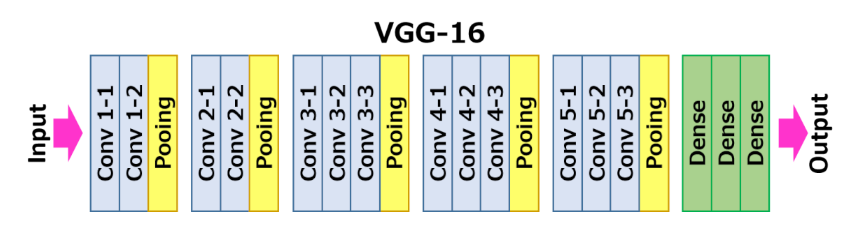
\includegraphics[width=3.0in]{figs/vgg-16}
	\caption{A listing of the layers involved in the VGG-16 Convolutional Neural Network Model.\cite{simonyan2014very}}
	\end{center}
\end{figure}
	


\section{Evaluation}
The machine learning solution apply feature extraction the neural network to replace the SIFT algorithm that find the interesting features in given images, after normalize the features, we train the feature regression neural networks with our datasets.\\
The feature regression takes in the sets of features between the two input images and predict the best parameters of the affine transformation instead of applying RANSAC which performs random sampling the regression over and over again to find the fit best parameters.\\
The machine learning algorithm takes the benefit that the machine can learn the transform of the images over times, compare to the SIFT and RANSAC that will have to start fresh whenever it gets the new images, the machine can speed by the process  training properly.\\
The goal is to evaluate the solution by comparing it against existing solutions, such as SIFT / RANSAC or manual alignment.











